\documentclass{article}
\usepackage{graphicx}
\usepackage{fancyhdr,extramarks}
\usepackage{enumitem}
\usepackage{amsmath}
\usepackage{amssymb}
\usepackage{xcolor, soul}
\usepackage{blindtext}
\usepackage{titlesec}
\usepackage[titles]{tocloft}
\usepackage[titles]{tocloft}
\usepackage{url}
\usepackage{hyperref}

% Formatting
\topmargin=-0.40in
\evensidemargin=0in
\oddsidemargin=0in
\textwidth=6.5in
\textheight=9.0in
\headsep=0.25in
\linespread{1.1}
\setlength\parindent{24pt}

% Page layout
\pagestyle{fancy}
\lhead{\Title}
\chead{\Course}
\rhead{\Topic}
\cfoot{\thepage}
\renewcommand\headrulewidth{0.4pt}
\renewcommand\footrulewidth{0.0pt}

\newcommand{\Title}{Final Project Report}
\newcommand{\Course}{{\bf 01:960:486}}
\newcommand{\Topic}{Nilay, Katharina, HaoYang, Rajeev}

\begin{document}

\section*{Introductory Description/Data Cleaning}
\hspace{\parindent} 

    The data set \href{https://archive.ics.uci.edu/dataset/2/adult}{adult} from UC Irvine's Machine Learning Repository in 1996 was extracted from the 1994 Census database, with a total of 15 variables to predict whether an individual's annual income exceeds $\$50$k

    The 15 variables were respectively: \texttt{age, workclass, fnlwgt, education, educationnum, $\linebreak$ martialstatus, occupation, relationship, race, sex, capitalgain, capitalloss, hoursperweek, nativecountry, 50k}

    First, we removed variables \texttt{capitalgain, capitalloss} simply due to most observations having missing values for them, then we removed variables \texttt{fnlwgt} as we note \href{https://www.kaggle.com/datasets/uciml/adult-census-income}{here}, \texttt{fnlwgt} being heavily determined by \texttt{age} and \texttt{sex} will produce high multicollinearity. We removed \texttt{education} for the same reason, as it's simply categorical representations of \texttt{educationnum}. We then removed \texttt{relationship} as it also causes multicollinearity with \texttt{sex}, as husband/wife would be associated with male/female. We removed \texttt{race} as its categories were too broad for us to expect significant findings. We lastly removed \texttt{nativecountry} simply because there are too many different categorical responses, with some holding so few observations while the variable itself has many missing values. 

     For further data cleaning, we first re-coded \texttt{sex, 50k} to binary variables, and \textbf{Federal-gov, Local-gov, State-gov} under \texttt{workclass} all to \textbf{gov}. We then added $3$ to every observation in \texttt{educationnum}, the $\#$ of years an individual spent in education, as it was strangely counting 3 years less (for example 10th grade in \texttt{education} only having \texttt{educationnum} of 7). Lastly, we removed the observations that have missing values in \texttt{workclass, occupation}, further the 21 observations with responses \textbf{Never-worked} and \textbf{Without-pay}, the dataset still has 30703 observations after data cleaning.

\section*{Exploratory Data Analysis}
    \subsection*{Outlier Detection}
    \hspace{\parindent} 

    As we are predicting a binary variable, we can't easily find outliers numerical for the response variable, so we look at the 3 numerical features, \texttt{age}, \texttt{educationnum}, and \texttt{hoursperweek}. As we have more than 30000 observations from the census, we may confidently use standardized methods, we will also use the iqr test.
    
    The range for \texttt{age} is 17 to 90. First, we standardize the distribution, and we find 122 observations with absolute values of $z$-scores larger than 3 with their ages ranging 78 to 90. Then, we find 172 observations that fall outside of the range of $(q1-1.5(\text{iqr}), q3+1.5(\text{iqr}))$ with the range being 76 to 90. As we have lots of observations, while most of the suspected outliers are overlapped, we will use the iqr test's set of suspected outliers, we then observe its histogram before and after removing the suspected outliers, here are the results:
    \begin{center}
    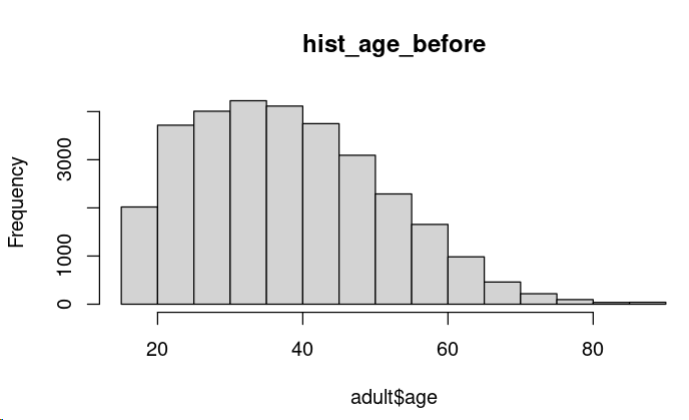
\includegraphics[scale = 0.3]{hist_age_before.png}
    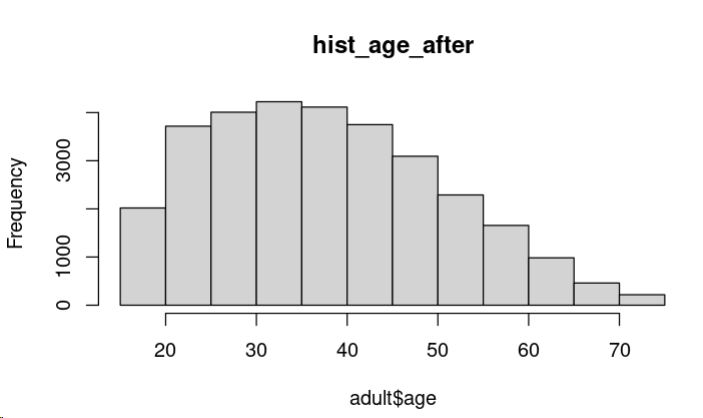
\includegraphics[scale = 0.3]{hist_age_after.png}
    \end{center}
    
    The range for \texttt{educationnum} is 4 to 19, with 19 being the standard number of years of education for someone with a doctorate degree. We find the exact same 202 observations that have 4 or 5 years of education to be the outliers under both the standardized $z$ test and the iqr test, we may observe the histograms from before and after removing the suspected outliers:
    \begin{center}
    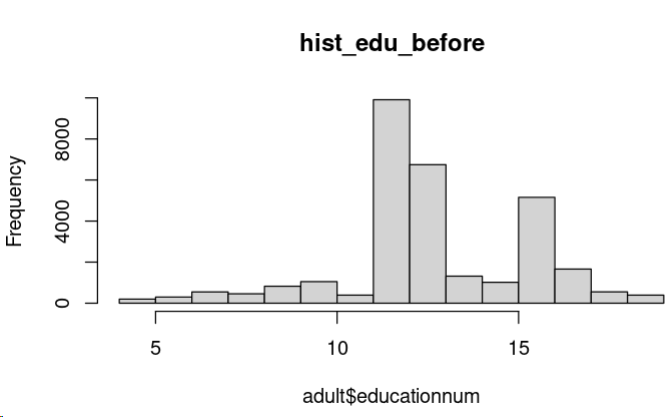
\includegraphics[scale = 0.3]{hist_edu_before.png}
    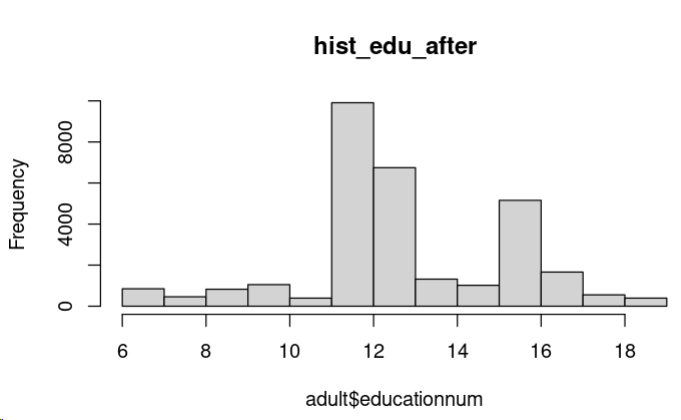
\includegraphics[scale = 0.3]{hist_edu_after.png}
    \end{center}

    The range for \texttt{hoursperweek} is 1 to 99, We find 450 observations that take values in $[1, 4] \cup [77, 99]$ through the standardized $z$ test, but through the iqr test, we find a total of 8092 observations that take value in 74 out of the original data's 94 unique values to be potential outliers. Although we wouldn't expect 450 potential outliers to heavily impact the data, 8092 is concerning. We find that $\mu \approx 41$ while $q2 = 40$, we may temporarily assign the cause of this being the distribution of \texttt{hoursperweek} having high kurtosis. We will look at the histograms after removing the different subsets of suspected outliers:

    \begin{center}
    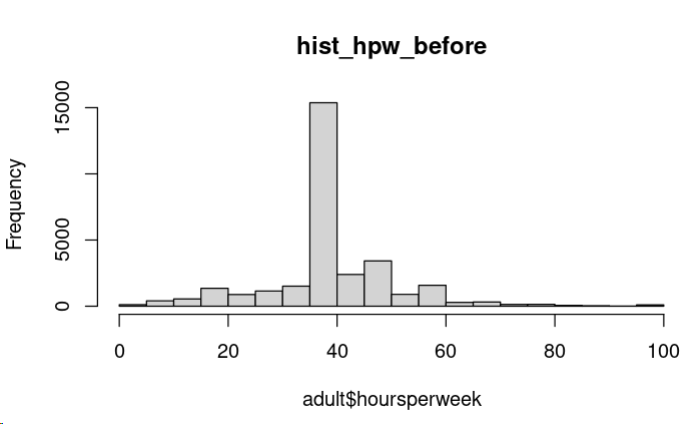
\includegraphics[scale = 0.22]{hist_hpw_before.png}
    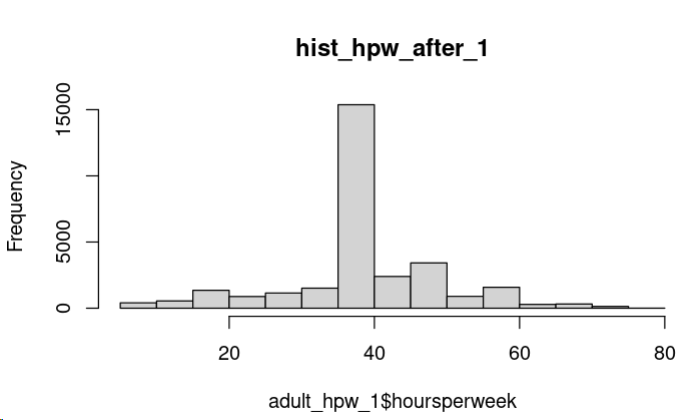
\includegraphics[scale = 0.22]{hist_hpw_after_1.png}
    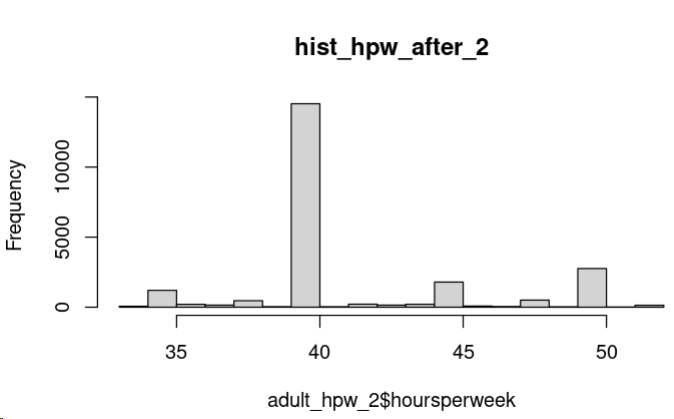
\includegraphics[scale = 0.22]{hist_hpw_after_2.png}
    \end{center}

    We note that distributions for both \texttt{age} and \texttt{educationnum} are seemingly more normally distributed for removing this little number of observations, thus we will keep these changes. For \texttt{hoursperweek}, we note that with the high percentage of data suspected as outliers by the iqr test, hist$\_$hpw$\_$after$\_$2 may be too extreme for not too significant result as we note \texttt{hoursperweek} equals to 40 for 14522 of the observations, near half, thus removing further beyond hist$\_$hpw$\_$after$\_$1 may unnecessarily erase reasonable spread useful for further analysis later.  

    There are still 29895 observations remaining after removing the suspected outliers, from which we may note that there are few overlaps. Further analysis will continue from here.
    
    \subsection*{Summary Statistics}
    \hspace{\parindent} 

    
    \subsection*{Data Visualization}
    \hspace{\parindent} 

    
\section*{Prediction Algorithms/Results}
    \subsection*{Support Vector Machines (SVN)}
    \hspace{\parindent} 


    \subsection*{Random Forest}
    \hspace{\parindent} 

    
\section*{Qualitative Discussion}
\hspace{\parindent} 

    
\end{document}
